% Options for packages loaded elsewhere
\PassOptionsToPackage{unicode}{hyperref}
\PassOptionsToPackage{hyphens}{url}
\PassOptionsToPackage{dvipsnames,svgnames,x11names}{xcolor}
%
\documentclass[
  letterpaper,
  DIV=11,
  numbers=noendperiod]{scrreprt}

\usepackage{amsmath,amssymb}
\usepackage{iftex}
\ifPDFTeX
  \usepackage[T1]{fontenc}
  \usepackage[utf8]{inputenc}
  \usepackage{textcomp} % provide euro and other symbols
\else % if luatex or xetex
  \usepackage{unicode-math}
  \defaultfontfeatures{Scale=MatchLowercase}
  \defaultfontfeatures[\rmfamily]{Ligatures=TeX,Scale=1}
\fi
\usepackage{lmodern}
\ifPDFTeX\else  
    % xetex/luatex font selection
\fi
% Use upquote if available, for straight quotes in verbatim environments
\IfFileExists{upquote.sty}{\usepackage{upquote}}{}
\IfFileExists{microtype.sty}{% use microtype if available
  \usepackage[]{microtype}
  \UseMicrotypeSet[protrusion]{basicmath} % disable protrusion for tt fonts
}{}
\makeatletter
\@ifundefined{KOMAClassName}{% if non-KOMA class
  \IfFileExists{parskip.sty}{%
    \usepackage{parskip}
  }{% else
    \setlength{\parindent}{0pt}
    \setlength{\parskip}{6pt plus 2pt minus 1pt}}
}{% if KOMA class
  \KOMAoptions{parskip=half}}
\makeatother
\usepackage{xcolor}
\setlength{\emergencystretch}{3em} % prevent overfull lines
\setcounter{secnumdepth}{5}
% Make \paragraph and \subparagraph free-standing
\makeatletter
\ifx\paragraph\undefined\else
  \let\oldparagraph\paragraph
  \renewcommand{\paragraph}{
    \@ifstar
      \xxxParagraphStar
      \xxxParagraphNoStar
  }
  \newcommand{\xxxParagraphStar}[1]{\oldparagraph*{#1}\mbox{}}
  \newcommand{\xxxParagraphNoStar}[1]{\oldparagraph{#1}\mbox{}}
\fi
\ifx\subparagraph\undefined\else
  \let\oldsubparagraph\subparagraph
  \renewcommand{\subparagraph}{
    \@ifstar
      \xxxSubParagraphStar
      \xxxSubParagraphNoStar
  }
  \newcommand{\xxxSubParagraphStar}[1]{\oldsubparagraph*{#1}\mbox{}}
  \newcommand{\xxxSubParagraphNoStar}[1]{\oldsubparagraph{#1}\mbox{}}
\fi
\makeatother

\usepackage{color}
\usepackage{fancyvrb}
\newcommand{\VerbBar}{|}
\newcommand{\VERB}{\Verb[commandchars=\\\{\}]}
\DefineVerbatimEnvironment{Highlighting}{Verbatim}{commandchars=\\\{\}}
% Add ',fontsize=\small' for more characters per line
\usepackage{framed}
\definecolor{shadecolor}{RGB}{241,243,245}
\newenvironment{Shaded}{\begin{snugshade}}{\end{snugshade}}
\newcommand{\AlertTok}[1]{\textcolor[rgb]{0.68,0.00,0.00}{#1}}
\newcommand{\AnnotationTok}[1]{\textcolor[rgb]{0.37,0.37,0.37}{#1}}
\newcommand{\AttributeTok}[1]{\textcolor[rgb]{0.40,0.45,0.13}{#1}}
\newcommand{\BaseNTok}[1]{\textcolor[rgb]{0.68,0.00,0.00}{#1}}
\newcommand{\BuiltInTok}[1]{\textcolor[rgb]{0.00,0.23,0.31}{#1}}
\newcommand{\CharTok}[1]{\textcolor[rgb]{0.13,0.47,0.30}{#1}}
\newcommand{\CommentTok}[1]{\textcolor[rgb]{0.37,0.37,0.37}{#1}}
\newcommand{\CommentVarTok}[1]{\textcolor[rgb]{0.37,0.37,0.37}{\textit{#1}}}
\newcommand{\ConstantTok}[1]{\textcolor[rgb]{0.56,0.35,0.01}{#1}}
\newcommand{\ControlFlowTok}[1]{\textcolor[rgb]{0.00,0.23,0.31}{\textbf{#1}}}
\newcommand{\DataTypeTok}[1]{\textcolor[rgb]{0.68,0.00,0.00}{#1}}
\newcommand{\DecValTok}[1]{\textcolor[rgb]{0.68,0.00,0.00}{#1}}
\newcommand{\DocumentationTok}[1]{\textcolor[rgb]{0.37,0.37,0.37}{\textit{#1}}}
\newcommand{\ErrorTok}[1]{\textcolor[rgb]{0.68,0.00,0.00}{#1}}
\newcommand{\ExtensionTok}[1]{\textcolor[rgb]{0.00,0.23,0.31}{#1}}
\newcommand{\FloatTok}[1]{\textcolor[rgb]{0.68,0.00,0.00}{#1}}
\newcommand{\FunctionTok}[1]{\textcolor[rgb]{0.28,0.35,0.67}{#1}}
\newcommand{\ImportTok}[1]{\textcolor[rgb]{0.00,0.46,0.62}{#1}}
\newcommand{\InformationTok}[1]{\textcolor[rgb]{0.37,0.37,0.37}{#1}}
\newcommand{\KeywordTok}[1]{\textcolor[rgb]{0.00,0.23,0.31}{\textbf{#1}}}
\newcommand{\NormalTok}[1]{\textcolor[rgb]{0.00,0.23,0.31}{#1}}
\newcommand{\OperatorTok}[1]{\textcolor[rgb]{0.37,0.37,0.37}{#1}}
\newcommand{\OtherTok}[1]{\textcolor[rgb]{0.00,0.23,0.31}{#1}}
\newcommand{\PreprocessorTok}[1]{\textcolor[rgb]{0.68,0.00,0.00}{#1}}
\newcommand{\RegionMarkerTok}[1]{\textcolor[rgb]{0.00,0.23,0.31}{#1}}
\newcommand{\SpecialCharTok}[1]{\textcolor[rgb]{0.37,0.37,0.37}{#1}}
\newcommand{\SpecialStringTok}[1]{\textcolor[rgb]{0.13,0.47,0.30}{#1}}
\newcommand{\StringTok}[1]{\textcolor[rgb]{0.13,0.47,0.30}{#1}}
\newcommand{\VariableTok}[1]{\textcolor[rgb]{0.07,0.07,0.07}{#1}}
\newcommand{\VerbatimStringTok}[1]{\textcolor[rgb]{0.13,0.47,0.30}{#1}}
\newcommand{\WarningTok}[1]{\textcolor[rgb]{0.37,0.37,0.37}{\textit{#1}}}

\providecommand{\tightlist}{%
  \setlength{\itemsep}{0pt}\setlength{\parskip}{0pt}}\usepackage{longtable,booktabs,array}
\usepackage{calc} % for calculating minipage widths
% Correct order of tables after \paragraph or \subparagraph
\usepackage{etoolbox}
\makeatletter
\patchcmd\longtable{\par}{\if@noskipsec\mbox{}\fi\par}{}{}
\makeatother
% Allow footnotes in longtable head/foot
\IfFileExists{footnotehyper.sty}{\usepackage{footnotehyper}}{\usepackage{footnote}}
\makesavenoteenv{longtable}
\usepackage{graphicx}
\makeatletter
\def\maxwidth{\ifdim\Gin@nat@width>\linewidth\linewidth\else\Gin@nat@width\fi}
\def\maxheight{\ifdim\Gin@nat@height>\textheight\textheight\else\Gin@nat@height\fi}
\makeatother
% Scale images if necessary, so that they will not overflow the page
% margins by default, and it is still possible to overwrite the defaults
% using explicit options in \includegraphics[width, height, ...]{}
\setkeys{Gin}{width=\maxwidth,height=\maxheight,keepaspectratio}
% Set default figure placement to htbp
\makeatletter
\def\fps@figure{htbp}
\makeatother

\usepackage{cancel}
\KOMAoption{captions}{tableheading}
\makeatletter
\@ifpackageloaded{tcolorbox}{}{\usepackage[skins,breakable]{tcolorbox}}
\@ifpackageloaded{fontawesome5}{}{\usepackage{fontawesome5}}
\definecolor{quarto-callout-color}{HTML}{909090}
\definecolor{quarto-callout-note-color}{HTML}{0758E5}
\definecolor{quarto-callout-important-color}{HTML}{CC1914}
\definecolor{quarto-callout-warning-color}{HTML}{EB9113}
\definecolor{quarto-callout-tip-color}{HTML}{00A047}
\definecolor{quarto-callout-caution-color}{HTML}{FC5300}
\definecolor{quarto-callout-color-frame}{HTML}{acacac}
\definecolor{quarto-callout-note-color-frame}{HTML}{4582ec}
\definecolor{quarto-callout-important-color-frame}{HTML}{d9534f}
\definecolor{quarto-callout-warning-color-frame}{HTML}{f0ad4e}
\definecolor{quarto-callout-tip-color-frame}{HTML}{02b875}
\definecolor{quarto-callout-caution-color-frame}{HTML}{fd7e14}
\makeatother
\makeatletter
\@ifpackageloaded{bookmark}{}{\usepackage{bookmark}}
\makeatother
\makeatletter
\@ifpackageloaded{caption}{}{\usepackage{caption}}
\AtBeginDocument{%
\ifdefined\contentsname
  \renewcommand*\contentsname{Table of contents}
\else
  \newcommand\contentsname{Table of contents}
\fi
\ifdefined\listfigurename
  \renewcommand*\listfigurename{List of Figures}
\else
  \newcommand\listfigurename{List of Figures}
\fi
\ifdefined\listtablename
  \renewcommand*\listtablename{List of Tables}
\else
  \newcommand\listtablename{List of Tables}
\fi
\ifdefined\figurename
  \renewcommand*\figurename{Figure}
\else
  \newcommand\figurename{Figure}
\fi
\ifdefined\tablename
  \renewcommand*\tablename{Table}
\else
  \newcommand\tablename{Table}
\fi
}
\@ifpackageloaded{float}{}{\usepackage{float}}
\floatstyle{ruled}
\@ifundefined{c@chapter}{\newfloat{codelisting}{h}{lop}}{\newfloat{codelisting}{h}{lop}[chapter]}
\floatname{codelisting}{Listing}
\newcommand*\listoflistings{\listof{codelisting}{List of Listings}}
\makeatother
\makeatletter
\makeatother
\makeatletter
\@ifpackageloaded{caption}{}{\usepackage{caption}}
\@ifpackageloaded{subcaption}{}{\usepackage{subcaption}}
\makeatother

\ifLuaTeX
  \usepackage{selnolig}  % disable illegal ligatures
\fi
\usepackage{bookmark}

\IfFileExists{xurl.sty}{\usepackage{xurl}}{} % add URL line breaks if available
\urlstyle{same} % disable monospaced font for URLs
\hypersetup{
  pdftitle={Time Series Analysis},
  pdfauthor={Yair Mau},
  colorlinks=true,
  linkcolor={blue},
  filecolor={Maroon},
  citecolor={Blue},
  urlcolor={Blue},
  pdfcreator={LaTeX via pandoc}}


\title{Time Series Analysis}
\author{Yair Mau}
\date{}

\begin{document}
\maketitle

\renewcommand*\contentsname{Table of contents}
{
\hypersetup{linkcolor=}
\setcounter{tocdepth}{2}
\tableofcontents
}

\bookmarksetup{startatroot}

\chapter*{about}\label{about}
\addcontentsline{toc}{chapter}{about}

\markboth{about}{about}

Welcome to \textbf{Time Series Analysis for Environmental Sciences}
(71106) at the Hebrew University of Jerusalem. This is Yair Mau, your
host for today. I am a senior lecturer at the Institute of Environmental
Sciences, at the Faculty of Agriculture, Food and Environment, in
Rehovot, Israel.

This website contains (almost) all the material you'll need for the
course. If you find any mistakes, or have any comments, please email me.

\section*{disclaimer}\label{disclaimer}
\addcontentsline{toc}{section}{disclaimer}

\markright{disclaimer}

The material here is not comprehensive and \texttt{does\ not} constitute
a stand alone course in Time Series Analysis. This is only the support
material for the actual presential course I give.

\section*{what, who, when and where?}\label{what-who-when-and-where}
\addcontentsline{toc}{section}{what, who, when and where?}

\markright{what, who, when and where?}

Course number 71106, 3 academic points\\
Yair Mau (lecturer), Erez Feuer (TA)\\
Tuesdays, from 11:15 to 14:00\\
Computer \href{https://goo.gl/maps/rzniv9NuyEs4ETH58}{classroom \#18}\\
Office hours: Tuesdays, from 09:45 to 10:45 (you should send an email to
let me know you are coming)

\section*{syllabus}\label{syllabus}
\addcontentsline{toc}{section}{syllabus}

\markright{syllabus}

\subsection*{course description}\label{course-description}
\addcontentsline{toc}{subsection}{course description}

Data analysis of time series, with practical examples from environmental
sciences.

\subsection*{course aims}\label{course-aims}
\addcontentsline{toc}{subsection}{course aims}

This course aims at giving the students a broad overview of the main
steps involved in the analysis of time series: data management, data
wrangling, visualization, analysis, and forecast. The course will
provide a hands-on approach, where students will actively engage with
real-life datasets from the field of environmental science.

\subsection*{learning outcomes}\label{learning-outcomes}
\addcontentsline{toc}{subsection}{learning outcomes}

On successful completion of this module,students should be able to:

\begin{itemize}
\tightlist
\item
  Explore a time-series dataset, while formulating interesting
  questions.
\item
  Choose the appropriate tools to attack the problem and answer the
  questions.
\item
  Communicate their findings and the methods they used to achieve them,
  using graphs, statistics, text, and a well-documented code.
\end{itemize}

\subsection*{course content}\label{course-content}
\addcontentsline{toc}{subsection}{course content}

\begin{itemize}
\tightlist
\item
  \textbf{Data wrangling:} organization, cleaning, merging, filling
  gaps, excluding outliers, smoothing, resampling.
\item
  \textbf{Visualization:} best practices for graph making using leading
  python libraries.
\item
  \textbf{Analysis:} stationarity, seasonality, (auto)correlations,
  lags, derivatives, spectral analysis.
\item
  \textbf{Forecast:} ARIMA
\item
  \textbf{Data management:} how to plan ahead and best organize large
  quantities of data. If there is enough time, we will build a simple
  time-series database.
\end{itemize}

\subsection*{books and other sources}\label{books-and-other-sources}
\addcontentsline{toc}{subsection}{books and other sources}

\href{references.html}{Click here.}

\subsection*{course evaluation}\label{course-evaluation}
\addcontentsline{toc}{subsection}{course evaluation}

There will be assignments during the semester (totaling 50\% of the
final grade), and one final project (50\%).

\subsection*{Evaluation policy}\label{evaluation-policy}
\addcontentsline{toc}{subsection}{Evaluation policy}

\begin{itemize}
\item
  \textbf{Individual Work:} While we support helping your peers, it's
  important to remember that all assignments must be completed
  individually. This means that your submissions should be your own
  unique work and not contain code or text that is identical to someone
  else's.
\item
  \textbf{Zero Plagiarism:} Do not copy text verbatim from any source.
  Always express ideas in your own words.
\item
  \textbf{On-Time Submission:} Assignments must be turned in by the
  specified deadline. Late submissions will receive a grade of 0. If you
  require an extension, requests will only be considered if made at
  least 24 hours before the due date.
\item
  \textbf{Non-Compliance Consequence:} Assignments that do not adhere to
  these guidelines will automatically receive a grade of 0.
\end{itemize}

\bookmarksetup{startatroot}

\chapter*{2024/2025 Schedule}\label{schedule}
\addcontentsline{toc}{chapter}{2024/2025 Schedule}

\markboth{2024/2025 Schedule}{2024/2025 Schedule}

\subsection*{Week 1, 29 Oct 2024}\label{week-1-29-oct-2024}
\addcontentsline{toc}{subsection}{Week 1, 29 Oct 2024}

\textbf{Introduction}

Course overview, setting of expectations, introduction to Jupyter
Notebooks, loading data and plotting it.

\href{assignments/assignment1}{Assignment 1}, due 12 Nov 2024

\subsection*{Week 2, 5 Nov 2024}\label{week-2-5-nov-2024}
\addcontentsline{toc}{subsection}{Week 2, 5 Nov 2024}

Resampling

\subsection*{Week 3, 12 Nov 2024}\label{week-3-12-nov-2024}
\addcontentsline{toc}{subsection}{Week 3, 12 Nov 2024}

Smoothing

\href{assignments/assignment2}{Assignment 2}, due 26 Nov 2024

\subsection*{Week 4, 19 Nov 2024}\label{week-4-19-nov-2024}
\addcontentsline{toc}{subsection}{Week 4, 19 Nov 2024}

Outliers

\subsection*{Week 5, 26 Nov 2024}\label{week-5-26-nov-2024}
\addcontentsline{toc}{subsection}{Week 5, 26 Nov 2024}

Stationarity: random processes, statistics refresher, AR processes

\href{assignments/assignment3}{Assignment 3}, due 10 Dec 2024

\subsection*{Week 6, 3 Dec 2024}\label{week-6-3-dec-2024}
\addcontentsline{toc}{subsection}{Week 6, 3 Dec 2024}

Stationarity: ACF and PACF graphs

\subsection*{Week 7, 10 Dec 2024}\label{week-7-10-dec-2024}
\addcontentsline{toc}{subsection}{Week 7, 10 Dec 2024}

Stationarity: Forecasting, ARIMA, SARIMA, SARIMAX

\href{assignments/assignment4}{Assignment 4}, due 31 Dec 2024

\subsection*{Week 8, 17 Dec 2024}\label{week-8-17-dec-2024}
\addcontentsline{toc}{subsection}{Week 8, 17 Dec 2024}

Seasonality

\subsection*{24 Dec 2024}\label{dec-2024}
\addcontentsline{toc}{subsection}{24 Dec 2024}

{No classes.}

\subsection*{Week 9, 31 Dec 2024}\label{week-9-31-dec-2024}
\addcontentsline{toc}{subsection}{Week 9, 31 Dec 2024}

\href{assignments/assignment5}{Assignment 5}, due 14 Jan 2025

\subsection*{Week 10, 7 Jan 2025}\label{week-10-7-jan-2025}
\addcontentsline{toc}{subsection}{Week 10, 7 Jan 2025}

\subsection*{Week 11, 14 Jan 2025}\label{week-11-14-jan-2025}
\addcontentsline{toc}{subsection}{Week 11, 14 Jan 2025}

\href{assignments/assignment6}{Assignment 6}, due 28 Jan 2025

\subsection*{Week 12, 21 Jan 2025}\label{week-12-21-jan-2025}
\addcontentsline{toc}{subsection}{Week 12, 21 Jan 2025}

\subsection*{Week 13, 28 Jan 2025}\label{week-13-28-jan-2025}
\addcontentsline{toc}{subsection}{Week 13, 28 Jan 2025}

\href{assignments/final-project}{Final project}, due 4 Mar 2025

\bookmarksetup{startatroot}

\chapter*{who cares?}\label{who-cares}
\addcontentsline{toc}{chapter}{who cares?}

\markboth{who cares?}{who cares?}

\section*{why ``Time Series Analysis?''}\label{why-time-series-analysis}
\addcontentsline{toc}{section}{why ``Time Series Analysis?''}

\markright{why ``Time Series Analysis?''}

Time has two aspects. There is the arrow, the running river, without
which there is no change, no progress, or direction, or creation. And
there is the circle or the cycle, without which there is chaos,
meaningless succession of instants, a world without clocks or seasons or
promises.\\
URSULA K. LE GUIN

You are here because you are interested in how things change, evolve. In
this course I want to discuss with you how to make sense of data whose
temporal nature is in its very essence. We will talk about randomness,
cycles, frequencies, correlations, and more.

\section*{why ``Environmental
Sciences''}\label{why-environmental-sciences}
\addcontentsline{toc}{section}{why ``Environmental Sciences''}

\markright{why ``Environmental Sciences''}

This same time series analysis (TSA) course could be called instead
``TSA for finance'', ``TSA for Biology'', or any other application. The
emphasis in this course is \textbf{not} Environmental Sciences, but the
concepts and tools of TSA. Because my research is in Environmental
Science, and many of the graduate students at HUJI-Rehovot research
this, I chose to use examples ``close to home''. The same toolset should
be useful for students of other disciplines.

\section*{what is it good for?}\label{what-is-it-good-for}
\addcontentsline{toc}{section}{what is it good for?}

\markright{what is it good for?}

In many fields of science we are flooded by data, and it's hard to see
the forest for the trees. I hope that the topics we'll discuss in this
course can help you find meaningful patterns in your data, formulate
interesting hypotheses, and design better experiments.

\section*{do I need it?}\label{do-i-need-it}
\addcontentsline{toc}{section}{do I need it?}

\markright{do I need it?}

Maybe. If you are a grad student and you have temporal data to analyze,
then probably yes. However, I have very fond memories of courses that I
took as a grad student that were completely unrelated to my research.
Sometimes ``because it's fun'' is a perfectly good answer.

\section*{\texorpdfstring{what will I \textbf{actually} gain from
it?}{what will I actually gain from it?}}\label{what-will-i-actually-gain-from-it}
\addcontentsline{toc}{section}{what will I \textbf{actually} gain from
it?}

\markright{what will I \textbf{actually} gain from it?}

By the end of this course you will have gained:

\begin{itemize}
\tightlist
\item
  a \textbf{hands-on} experience of fundamental time-series analysis
  tools
\item
  an \textbf{intuition} regarding the basic concepts
\item
  \textbf{technical} abilities
\item
  a \textbf{springboard} for learning more about the subject by yourself
\end{itemize}

\part{start here}

\chapter{the boring stuff you absolutely need to
do}\label{the-boring-stuff-you-absolutely-need-to-do}

I assume everyone registered has taken a basic Python course. On your
computer, do the following:

\section{Anaconda}\label{anaconda}

Install \href{https://www.anaconda.com/download}{Anaconda's Python
distribution}. The Anaconda installation brings with it all the main
python packages we will need to use. In order to install extra packages,
refer to these two tutorials:
\href{https://www.tutorialspoint.com/how-do-i-install-python-packages-in-anaconda}{tutorial
1},
\href{https://docs.anaconda.com/free/anaconda/packages/install-packages.html}{tutorial
2}.

\section{VSCode}\label{vscode}

Install \href{https://code.visualstudio.com/download}{VSCode}. Visual
Studio Code is a very nice IDE (Integrated Development Environment) made
by Microsoft, available to all operating systems. Contrary to the title
of this page, it is not absolutely necessary to use it, but I like
VSCode, and as my student, so do you 😉.

\section{jupyter notebooks}\label{jupyter-notebooks}

We will code exclusively in Jupyter Notebooks.
\href{https://code.visualstudio.com/docs/datascience/jupyter-notebooks}{Get
acquainted with them}. Make sure you can
\href{https://opensourceoptions.com/blog/setup-anaconda-python-to-work-with-visual-studio-code-on-windows/}{point
VSCode} to the Anaconda environment of your choice (``base'' by
default). Don't worry, this is easier than it sounds.

One failproof way of making sure VSCode uses the Anaconda installation
is the following:

\begin{itemize}
\tightlist
\item
  Open Anaconda Navigator
\item
  If you are using HUJI's computers, in ``Environments'', choose
  ``asgard''. If you are using your own computer, ignore this step.
\item
  open VSCode from inside Anaconda Navigator (see image below).
\end{itemize}

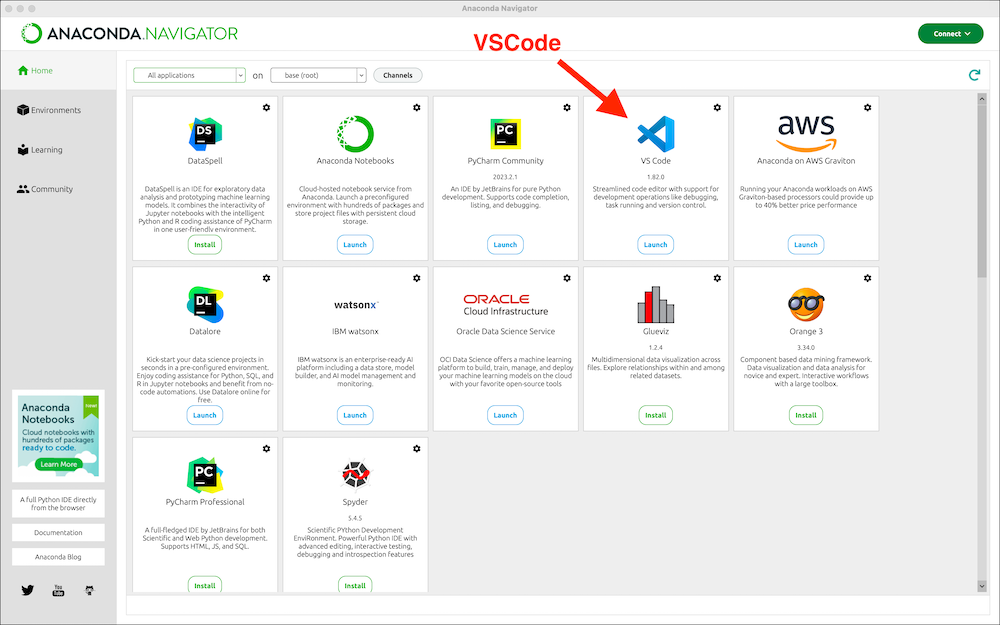
\includegraphics{basics/./anacondanavigator.png}

Sometimes you will need to manualy install the Jupyter extension on
VSCode. In this case follow
\href{https://code.visualstudio.com/docs/datascience/jupyter-notebooks}{this
tutorial}.

\section{folder structure}\label{folder-structure}

You \textbf{NEED} to be confortable with you computer's folder (or
directory) structure. Where are files located? How to navigate through
different folders? How is my stuff organized? If you don't feel
\textbf{absolutely} comfortable with this, then read this,
\href{http://www2.westsussex.gov.uk/LearningandDevelopment/IT\%20Learning\%20Guides/Microsoft\%20Windows\%207/05\%20Working\%20with\%20folders.pdf}{Windows},
\href{https://recoverit.wondershare.com/mac-tips/mac-finder-tutorial-mac.html}{MacOS}.
If you use Linux then you surely know this stuff. \textbf{Make yourself
a ``time-series'' folder} wherever you want, and have it backed up
regularly (use Google Drive, Dropbox, do it manually, etc). ``My dog
deleted my files'' is not an excuse.

\chapter{numpy, pandas, matplotlib}\label{numpy-pandas-matplotlib}

\begin{Shaded}
\begin{Highlighting}[]
\ImportTok{import}\NormalTok{ numpy }\ImportTok{as}\NormalTok{ np}
\ImportTok{import}\NormalTok{ pandas }\ImportTok{as}\NormalTok{ pd}
\ImportTok{import}\NormalTok{ matplotlib.pyplot }\ImportTok{as}\NormalTok{ plt}
\end{Highlighting}
\end{Shaded}

The three lines above are the most common way you will start every
project in this course.

\begin{itemize}
\tightlist
\item
  \textbf{numpy} = numerical python. This library has a ton useful
  mathematical functions, and most importantly, it has an object called
  \texttt{numpy\ array}, which is one of the most useful data structures
  we have for time series analysis.
\item
  \textbf{pandas} is built upon numpy, and allows us to easily
  manipulate data stored in \texttt{dataframes}, a fancy name for a
  table.
\item
  \textbf{pyplot} is a submodule of \texttt{matplotlib}, and allows us
  to beautifully plot data.
\end{itemize}

The best resource I know to get acquainted with all three packages is
\href{https://jakevdp.github.io/PythonDataScienceHandbook/index.html}{Python
Data Science Handbook, by Jake VanderPlas}. This is a free online book,
with excellent step by step examples.

\section{pandas}\label{pandas}

We will primarily use the Pandas package to deal with data. Pandas has
become the standard Python tool to manipulate time series, and you
should get acquainted with its basic usage. This course will provide you
the opportunity to learn by example, but I'm sure we will only scratch
the surface, and you'll be left with lots of questions.

I provide below a (non-comprehensive) list of useful tutorials, they are
a good reference for the beginner and for the experienced user.

\begin{itemize}
\tightlist
\item
  \href{https://jakevdp.github.io/PythonDataScienceHandbook/index.html}{Python
  Data Science Handbook, by Jake VanderPlas}
\item
  \href{https://pandas.pydata.org/Pandas_Cheat_Sheet.pdf}{Data Wrangling
  with pandas Cheat Sheet}
\item
  \href{https://images.datacamp.com/image/upload/v1666944896/Marketing/Blog/Working_with_Dates_and_Times_Cheat_Sheet.pdf}{Working
  with Dates and Times in Python}
\item
  \href{https://www.webpages.uidaho.edu/~stevel/cheatsheets/Pandas\%20DataFrame\%20Notes_12pages.pdf}{Cheat
  Sheet: The pandas DataFrame Object}
\item
  \href{https://www.youtube.com/watch?v=ZyhVh-qRZPA&list=PL-osiE80TeTsWmV9i9c58mdDCSskIFdDS&pp=iAQB}{YouTube
  tutorials} by Corey Schafer
\end{itemize}

\section{pyplot}\label{pyplot}

Matplotlib, and its submodule pyplot, are probably the most common
Python plotting tool. Pyplot is both great and horrible:

\begin{itemize}
\tightlist
\item
  Great: you'll have absolutely full control of everything you want to
  plot. The sky is the limit.
\item
  Horrible: you'll cry as you do it, because there is so much to know,
  and it is not the most friendly plotting package.
\end{itemize}

Pyplot is \emph{object oriented}, so you will usually manipulate the
\textbf{axes} object like this.

\begin{Shaded}
\begin{Highlighting}[]
\ImportTok{import}\NormalTok{ matplotlib.pyplot }\ImportTok{as}\NormalTok{ plt}

\NormalTok{x }\OperatorTok{=}\NormalTok{ [}\DecValTok{1}\NormalTok{, }\DecValTok{2}\NormalTok{, }\DecValTok{3}\NormalTok{, }\DecValTok{4}\NormalTok{, }\DecValTok{5}\NormalTok{]}
\NormalTok{y }\OperatorTok{=}\NormalTok{ [}\DecValTok{1}\NormalTok{, }\DecValTok{4}\NormalTok{, }\DecValTok{2}\NormalTok{, }\DecValTok{0}\NormalTok{, }\DecValTok{3}\NormalTok{]}

\CommentTok{\# Figure with two plots}
\NormalTok{fig, (ax1, ax2) }\OperatorTok{=}\NormalTok{ plt.subplots(}\DecValTok{1}\NormalTok{, }\DecValTok{2}\NormalTok{, figsize }\OperatorTok{=}\NormalTok{ (}\DecValTok{8}\NormalTok{, }\DecValTok{6}\NormalTok{))}
\CommentTok{\# plot on the left}
\NormalTok{ax1.plot(x, y, color}\OperatorTok{=}\StringTok{"tab:blue"}\NormalTok{)}
\NormalTok{ax1.plot(x, y[::}\OperatorTok{{-}}\DecValTok{1}\NormalTok{], color}\OperatorTok{=}\StringTok{"tab:orange"}\NormalTok{)}
\NormalTok{ax1.}\BuiltInTok{set}\NormalTok{(xlabel}\OperatorTok{=}\StringTok{"date"}\NormalTok{,}
\NormalTok{        ylabel}\OperatorTok{=}\StringTok{"something"}\NormalTok{,}
\NormalTok{        title}\OperatorTok{=}\StringTok{"left panel"}\NormalTok{)}
\CommentTok{\# plot on the right}
\NormalTok{ax2.plot(x, y[::}\OperatorTok{{-}}\DecValTok{1}\NormalTok{])}
\NormalTok{ax2.}\BuiltInTok{set}\NormalTok{(xlabel}\OperatorTok{=}\StringTok{"date"}\NormalTok{,}
\NormalTok{        ylabel}\OperatorTok{=}\StringTok{"something else"}\NormalTok{,}
\NormalTok{        title}\OperatorTok{=}\StringTok{"right panel"}\NormalTok{)}
\end{Highlighting}
\end{Shaded}

\begin{verbatim}
[Text(0.5, 0, 'date'),
 Text(0, 0.5, 'something else'),
 Text(0.5, 1.0, 'right panel')]
\end{verbatim}

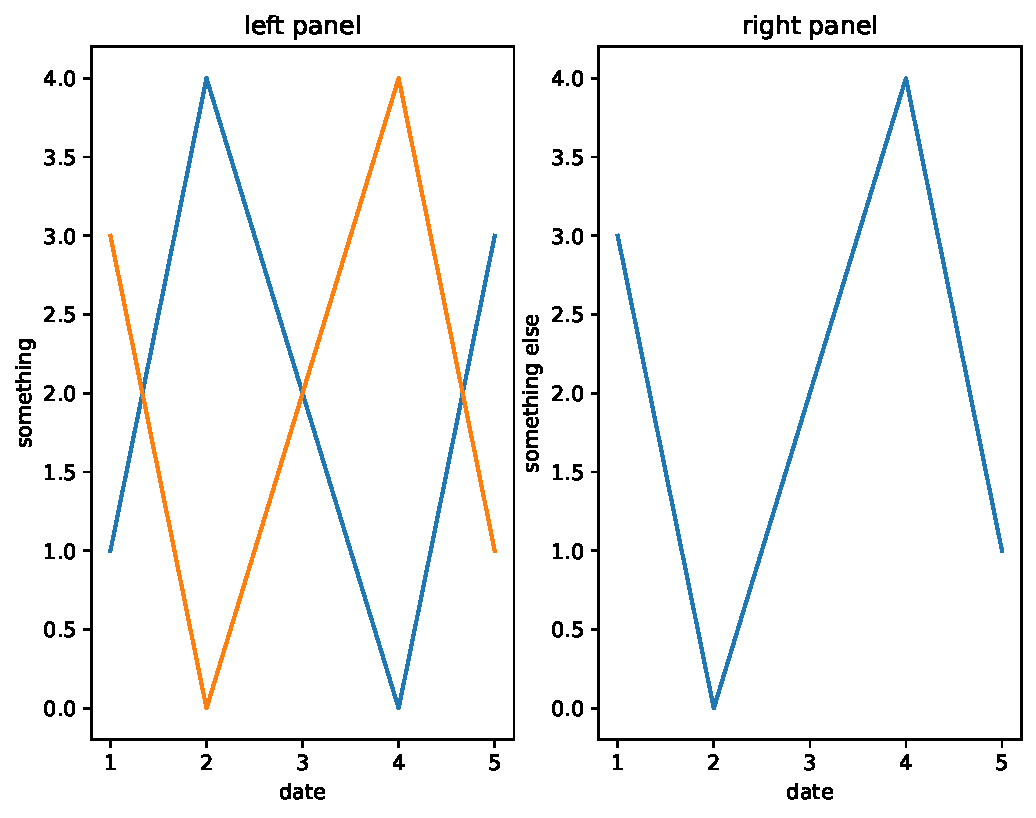
\includegraphics{basics/numpy-pandas-matplotlib_files/figure-pdf/cell-2-output-2.pdf}

For the very beginners, you need to know that \texttt{figure} refers to
the whole white canvas, and \texttt{axes} means the rectangle inside
which something will be plotted:

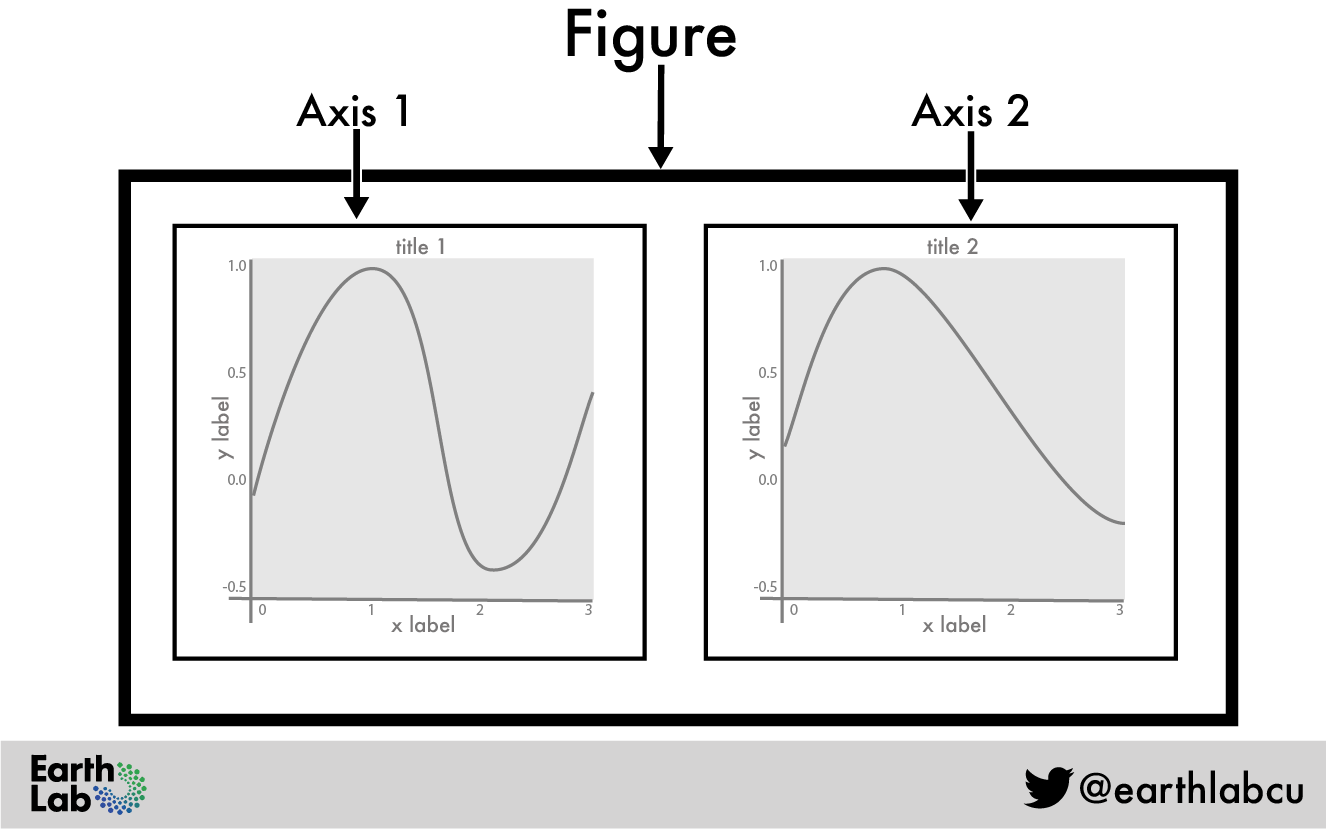
\includegraphics{basics/fig-2-plots.png}

The image above is good because it has 2 panels, and it's easy to
understand what going on. Sadly, they mixed the two terms, axis and
axes.

\begin{itemize}
\tightlist
\item
  \textbf{axes} is where the whole plot will be drawn. In the figure
  above it is the same as each panel.
\item
  \textbf{axis} is each of the vertical and horizontal lines, where you
  have ticks and numbers.
\end{itemize}

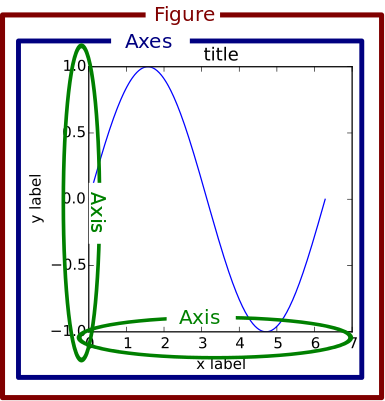
\includegraphics{basics/axis-vs-axes.png}

If you are new to all this, I recommend that you go to:

\begin{itemize}
\tightlist
\item
  \href{https://www.earthdatascience.org/courses/scientists-guide-to-plotting-data-in-python/plot-with-matplotlib/introduction-to-matplotlib-plots/}{Earth
  Lab's Introduction to Plotting in Python Using Matplotlib}
\item
  \href{https://jakevdp.github.io/PythonDataScienceHandbook/index.html}{Jake
  VanderPlas's Python Data Science Handbook}
\end{itemize}

\part{resampling}

\chapter{motivation}\label{motivation}

\section{Jerusalem, 2019}\label{jerusalem-2019}

Data from the \href{https://ims.gov.il/en/data_gov}{Israel
Meteorological Service}, IMS.

See the temperature at a weather station in Jerusalem, for the whole
2019 year. This is an interactive graph: to zoom in, play with the
bottom panel.

\begin{verbatim}
alt.VConcatChart(...)
\end{verbatim}

\paragraph*{\texorpdfstring{ discussion}{ discussion}}\label{discussion}
\addcontentsline{toc}{paragraph}{ discussion}

The temperature fluctuates on various time scales, from daily to yearly.
Let's think together a few questions we'd like to ask about the data
above.

Now let's see precipitation data:

\begin{verbatim}
alt.VConcatChart(...)
\end{verbatim}

\paragraph*{\texorpdfstring{
discussion}{ discussion}}\label{discussion-1}
\addcontentsline{toc}{paragraph}{ discussion}

What would be interesting to know about precipitation?

We have not talked about what kind of data we have in our hands here.
The csv file provided by the IMS looks like this:

\begin{longtable}[]{@{}lllllllllllllllllll@{}}
\toprule\noalign{}
& Station & Date \& Time (Winter) & Diffused radiation (W/m\^{}2) &
Global radiation (W/m\^{}2) & Direct radiation (W/m\^{}2) & Relative
humidity (\%) & Temperature (°C) & Maximum temperature (°C) & Minimum
temperature (°C) & Wind direction (°) & Gust wind direction (°) & Wind
speed (m/s) & Maximum 1 minute wind speed (m/s) & Maximum 10 minutes
wind speed (m/s) & Time ending maximum 10 minutes wind speed (hhmm) &
Gust wind speed (m/s) & Standard deviation wind direction (°) & Rainfall
(mm) \\
\midrule\noalign{}
\endhead
\bottomrule\noalign{}
\endlastfoot
0 & Jerusalem Givat Ram & 01/01/2019 00:00 & 0.0 & 0.0 & 0.0 & 80.0 &
8.7 & 8.8 & 8.6 & 75.0 & 84.0 & 3.3 & 4.3 & 3.5 & 23:58 & 6.0 & 15.6 &
0.0 \\
1 & Jerusalem Givat Ram & 01/01/2019 00:10 & 0.0 & 0.0 & 0.0 & 79.0 &
8.7 & 8.8 & 8.7 & 74.0 & 82.0 & 3.3 & 4.1 & 3.3 & 00:01 & 4.9 & 14.3 &
0.0 \\
2 & Jerusalem Givat Ram & 01/01/2019 00:20 & 0.0 & 0.0 & 0.0 & 79.0 &
8.7 & 8.8 & 8.7 & 76.0 & 82.0 & 3.2 & 4.1 & 3.3 & 00:19 & 4.9 & 9.9 &
0.0 \\
3 & Jerusalem Givat Ram & 01/01/2019 00:30 & 0.0 & 0.0 & 0.0 & 79.0 &
8.7 & 8.7 & 8.6 & 78.0 & 73.0 & 3.6 & 4.2 & 3.6 & 00:30 & 5.2 & 11.7 &
0.0 \\
4 & Jerusalem Givat Ram & 01/01/2019 00:40 & 0.0 & 0.0 & 0.0 & 79.0 &
8.6 & 8.7 & 8.5 & 80.0 & 74.0 & 3.6 & 4.4 & 3.8 & 00:35 & 5.4 & 10.5 &
0.0 \\
... & ... & ... & ... & ... & ... & ... & ... & ... & ... & ... & ... &
... & ... & ... & ... & ... & ... & ... \\
52549 & Jerusalem Givat Ram & 31/12/2019 22:20 & 0.0 & 0.0 & 1.0 & 81.0
& 7.4 & 7.6 & 7.3 & 222.0 & 255.0 & 0.5 & 0.9 & 1.0 & 22:11 & 1.0 & 47.9
& 0.0 \\
52550 & Jerusalem Givat Ram & 31/12/2019 22:30 & 0.0 & 0.0 & 1.0 & 83.0
& 7.3 & 7.4 & 7.3 & 266.0 & 259.0 & 0.6 & 0.8 & 0.6 & 22:28 & 1.1 & 22.8
& 0.0 \\
52551 & Jerusalem Givat Ram & 31/12/2019 22:40 & 0.0 & 0.0 & 1.0 & 83.0
& 7.5 & 7.6 & 7.3 & 331.0 & 317.0 & 0.5 & 0.8 & 0.6 & 22:35 & 1.0 & 31.6
& 0.0 \\
52552 & Jerusalem Givat Ram & 31/12/2019 22:50 & 0.0 & 0.0 & 1.0 & 83.0
& 7.5 & 7.6 & 7.4 & 312.0 & 285.0 & 0.6 & 1.0 & 0.6 & 22:50 & 1.4 & 31.3
& 0.0 \\
52553 & Jerusalem Givat Ram & 31/12/2019 23:00 & 0.0 & 0.0 & 1.0 & 83.0
& 7.6 & 7.7 & 7.4 & 315.0 & 321.0 & 0.7 & 1.0 & 0.8 & 22:54 & 1.3 & 23.5
& 0.0 \\
\end{longtable}

We see that we have data points spaced out evenly every 10 minutes.

\section{Challenges}\label{challenges}

Let's try to answer the following questions:

\begin{tcolorbox}[enhanced jigsaw, colbacktitle=quarto-callout-note-color!10!white, colback=white, title={What is the mean temperature for each month?}, colframe=quarto-callout-note-color-frame, opacityback=0, left=2mm, opacitybacktitle=0.6, breakable, bottomrule=.15mm, bottomtitle=1mm, toptitle=1mm, titlerule=0mm, arc=.35mm, rightrule=.15mm, toprule=.15mm, leftrule=.75mm, coltitle=black]

First we have to divide temperature data by month, and then take the
average for each month.

a possible solution

\begin{Shaded}
\begin{Highlighting}[]
\NormalTok{df\_month }\OperatorTok{=}\NormalTok{ df[}\StringTok{\textquotesingle{}temperature\textquotesingle{}}\NormalTok{].resample(}\StringTok{\textquotesingle{}M\textquotesingle{}}\NormalTok{).mean()}
\end{Highlighting}
\end{Shaded}

\end{tcolorbox}

\begin{tcolorbox}[enhanced jigsaw, colbacktitle=quarto-callout-note-color!10!white, colback=white, title={For each month, what is the mean of the daily maximum temperature? What
about the minimun?}, colframe=quarto-callout-note-color-frame, opacityback=0, left=2mm, opacitybacktitle=0.6, breakable, bottomrule=.15mm, bottomtitle=1mm, toptitle=1mm, titlerule=0mm, arc=.35mm, rightrule=.15mm, toprule=.15mm, leftrule=.75mm, coltitle=black]

This is a bit trickier.

\begin{enumerate}
\def\labelenumi{\arabic{enumi}.}
\tightlist
\item
  We need to find the maximum/minimum temperature for each day.
\item
  Only then we split the daily data by month and take the average.
\end{enumerate}

a possible solution

\begin{Shaded}
\begin{Highlighting}[]
\NormalTok{df\_day[}\StringTok{\textquotesingle{}max temp\textquotesingle{}}\NormalTok{] }\OperatorTok{=}\NormalTok{ df[}\StringTok{\textquotesingle{}temperature\textquotesingle{}}\NormalTok{].resample(}\StringTok{\textquotesingle{}D\textquotesingle{}}\NormalTok{).}\BuiltInTok{max}\NormalTok{()}
\NormalTok{df\_month[}\StringTok{\textquotesingle{}max temp\textquotesingle{}}\NormalTok{] }\OperatorTok{=}\NormalTok{ df\_day[}\StringTok{\textquotesingle{}max temp\textquotesingle{}}\NormalTok{].resample(}\StringTok{\textquotesingle{}MS\textquotesingle{}}\NormalTok{).mean()}
\end{Highlighting}
\end{Shaded}

\end{tcolorbox}

\begin{tcolorbox}[enhanced jigsaw, colbacktitle=quarto-callout-note-color!10!white, colback=white, title={What is the average night temperature for every season? What about the
day temperature?}, colframe=quarto-callout-note-color-frame, opacityback=0, left=2mm, opacitybacktitle=0.6, breakable, bottomrule=.15mm, bottomtitle=1mm, toptitle=1mm, titlerule=0mm, arc=.35mm, rightrule=.15mm, toprule=.15mm, leftrule=.75mm, coltitle=black]

\begin{enumerate}
\def\labelenumi{\arabic{enumi}.}
\tightlist
\item
  We need to filter our data to contain only night times.
\item
  We need to divide rain data by seasons (3 months), and then take the
  mean for each season.
\end{enumerate}

a possible solution

\begin{Shaded}
\begin{Highlighting}[]
\CommentTok{\# filter only night data}
\NormalTok{df\_night }\OperatorTok{=}\NormalTok{ df.loc[((df.index.hour }\OperatorTok{\textless{}} \DecValTok{6}\NormalTok{) }\OperatorTok{|}\NormalTok{ (df.index.hour }\OperatorTok{\textgreater{}=} \DecValTok{18}\NormalTok{))]}
\NormalTok{season\_average\_night\_temp }\OperatorTok{=}\NormalTok{ df\_night[}\StringTok{\textquotesingle{}temperature\textquotesingle{}}\NormalTok{].resample(}\StringTok{\textquotesingle{}Q\textquotesingle{}}\NormalTok{).mean()}
\end{Highlighting}
\end{Shaded}

another possible solution

\begin{Shaded}
\begin{Highlighting}[]
\CommentTok{\# filter using between\_time}
\NormalTok{df\_night }\OperatorTok{=}\NormalTok{ df.between\_time(}\StringTok{\textquotesingle{}18:00\textquotesingle{}}\NormalTok{, }\StringTok{\textquotesingle{}06:00\textquotesingle{}}\NormalTok{, inclusive}\OperatorTok{=}\StringTok{\textquotesingle{}left\textquotesingle{}}\NormalTok{)}
\NormalTok{season\_average\_night\_temp }\OperatorTok{=}\NormalTok{ df\_night[}\StringTok{\textquotesingle{}temperature\textquotesingle{}}\NormalTok{].resample(}\StringTok{\textquotesingle{}Q\textquotesingle{}}\NormalTok{).mean()}
\end{Highlighting}
\end{Shaded}

\end{tcolorbox}

\begin{tcolorbox}[enhanced jigsaw, colbacktitle=quarto-callout-note-color!10!white, colback=white, title={What is the daily precipitation?}, colframe=quarto-callout-note-color-frame, opacityback=0, left=2mm, opacitybacktitle=0.6, breakable, bottomrule=.15mm, bottomtitle=1mm, toptitle=1mm, titlerule=0mm, arc=.35mm, rightrule=.15mm, toprule=.15mm, leftrule=.75mm, coltitle=black]

First we have to divide rain data by day, and then take the sum for each
day.

a possible solution

\begin{Shaded}
\begin{Highlighting}[]
\NormalTok{daily\_precipitation }\OperatorTok{=}\NormalTok{ df[}\StringTok{\textquotesingle{}rain\textquotesingle{}}\NormalTok{].resample(}\StringTok{\textquotesingle{}D\textquotesingle{}}\NormalTok{).}\BuiltInTok{sum}\NormalTok{()}
\end{Highlighting}
\end{Shaded}

\end{tcolorbox}

\begin{tcolorbox}[enhanced jigsaw, colbacktitle=quarto-callout-note-color!10!white, colback=white, title={How much rain was there every month?}, colframe=quarto-callout-note-color-frame, opacityback=0, left=2mm, opacitybacktitle=0.6, breakable, bottomrule=.15mm, bottomtitle=1mm, toptitle=1mm, titlerule=0mm, arc=.35mm, rightrule=.15mm, toprule=.15mm, leftrule=.75mm, coltitle=black]

We have to divide rain data by month, and then sum the totals of each
month.

a possible solution

\begin{Shaded}
\begin{Highlighting}[]
\NormalTok{monthly\_precipitation }\OperatorTok{=}\NormalTok{ df[}\StringTok{\textquotesingle{}rain\textquotesingle{}}\NormalTok{].resample(}\StringTok{\textquotesingle{}M\textquotesingle{}}\NormalTok{).}\BuiltInTok{sum}\NormalTok{()}
\end{Highlighting}
\end{Shaded}

\end{tcolorbox}

\begin{tcolorbox}[enhanced jigsaw, colbacktitle=quarto-callout-note-color!10!white, colback=white, title={How many rainy days were there each month?}, colframe=quarto-callout-note-color-frame, opacityback=0, left=2mm, opacitybacktitle=0.6, breakable, bottomrule=.15mm, bottomtitle=1mm, toptitle=1mm, titlerule=0mm, arc=.35mm, rightrule=.15mm, toprule=.15mm, leftrule=.75mm, coltitle=black]

\begin{enumerate}
\def\labelenumi{\arabic{enumi}.}
\tightlist
\item
  We need to sum rain by day.
\item
  We need to count how many days are there each month where
  \texttt{rain\ \textgreater{}\ 0}.
\end{enumerate}

a possible solution

\begin{Shaded}
\begin{Highlighting}[]
\NormalTok{daily\_precipitation }\OperatorTok{=}\NormalTok{ df[}\StringTok{\textquotesingle{}rain\textquotesingle{}}\NormalTok{].resample(}\StringTok{\textquotesingle{}D\textquotesingle{}}\NormalTok{).}\BuiltInTok{sum}\NormalTok{()}
\NormalTok{only\_rainy\_days }\OperatorTok{=}\NormalTok{ daily\_precipitation.loc[daily\_precipitation }\OperatorTok{\textgreater{}} \DecValTok{0}\NormalTok{]}
\NormalTok{rain\_days\_per\_month }\OperatorTok{=}\NormalTok{ only\_rainy\_days.resample(}\StringTok{\textquotesingle{}M\textquotesingle{}}\NormalTok{).count()}
\end{Highlighting}
\end{Shaded}

\end{tcolorbox}

\begin{tcolorbox}[enhanced jigsaw, colbacktitle=quarto-callout-note-color!10!white, colback=white, title={How many days, hours, and minutes were between the last rain of the
season (Malkosh) to the first (Yoreh)?}, colframe=quarto-callout-note-color-frame, opacityback=0, left=2mm, opacitybacktitle=0.6, breakable, bottomrule=.15mm, bottomtitle=1mm, toptitle=1mm, titlerule=0mm, arc=.35mm, rightrule=.15mm, toprule=.15mm, leftrule=.75mm, coltitle=black]

\begin{enumerate}
\def\labelenumi{\arabic{enumi}.}
\tightlist
\item
  We need to divide our data into two: \texttt{rainy\_season\_1} and
  \texttt{rainy\_season\_2}.
\item
  We need to find the time of the last rain in
  \texttt{rainy\_season\_1}.
\item
  We need to find the time of the first rain in
  \texttt{rainy\_season\_2}.
\item
  We need to compute the time difference between the two dates.
\end{enumerate}

a possible solution

\begin{Shaded}
\begin{Highlighting}[]
\NormalTok{split\_date }\OperatorTok{=} \StringTok{\textquotesingle{}2019{-}08{-}01\textquotesingle{}}
\NormalTok{rainy\_season\_1 }\OperatorTok{=}\NormalTok{ df[:split\_date]  }\CommentTok{\# everything before split date}
\NormalTok{rainy\_season\_2 }\OperatorTok{=}\NormalTok{ df[split\_date:]  }\CommentTok{\# everything after split date}
\NormalTok{malkosh }\OperatorTok{=}\NormalTok{ rainy\_season\_1[}\StringTok{\textquotesingle{}rain\textquotesingle{}}\NormalTok{].loc[rainy\_season\_1[}\StringTok{\textquotesingle{}rain\textquotesingle{}}\NormalTok{] }\OperatorTok{\textgreater{}} \DecValTok{0}\NormalTok{].last\_valid\_index()}
\NormalTok{yoreh }\OperatorTok{=}\NormalTok{ rainy\_season\_2[}\StringTok{\textquotesingle{}rain\textquotesingle{}}\NormalTok{].loc[rainy\_season\_2[}\StringTok{\textquotesingle{}rain\textquotesingle{}}\NormalTok{] }\OperatorTok{\textgreater{}} \DecValTok{0}\NormalTok{].first\_valid\_index()}
\NormalTok{dry\_period }\OperatorTok{=}\NormalTok{ yoreh }\OperatorTok{{-}}\NormalTok{ malkosh}
\CommentTok{\# extracting days, hours, and minutes}
\NormalTok{days }\OperatorTok{=}\NormalTok{ dry\_period.days}
\NormalTok{hours }\OperatorTok{=}\NormalTok{ dry\_period.components.hours}
\NormalTok{minutes }\OperatorTok{=}\NormalTok{ dry\_period.components.minutes}
\BuiltInTok{print}\NormalTok{(}\SpecialStringTok{f\textquotesingle{}The dry period of 2019 was }\SpecialCharTok{\{}\NormalTok{days}\SpecialCharTok{\}}\SpecialStringTok{ days, }\SpecialCharTok{\{}\NormalTok{hours}\SpecialCharTok{\}}\SpecialStringTok{ hours and }\SpecialCharTok{\{}\NormalTok{minutes}\SpecialCharTok{\}}\SpecialStringTok{ minutes.\textquotesingle{}}\NormalTok{)}
\end{Highlighting}
\end{Shaded}

\end{tcolorbox}

\begin{tcolorbox}[enhanced jigsaw, colbacktitle=quarto-callout-note-color!10!white, colback=white, title=\textcolor{quarto-callout-note-color}{\faInfo}\hspace{0.5em}{What was the rainiest morning (6am-12pm) of the year? Bonus, what about
the rainiest night (6pm-6am)?}, colframe=quarto-callout-note-color-frame, opacityback=0, left=2mm, opacitybacktitle=0.6, breakable, bottomrule=.15mm, bottomtitle=1mm, toptitle=1mm, titlerule=0mm, arc=.35mm, rightrule=.15mm, toprule=.15mm, leftrule=.75mm, coltitle=black]

\begin{enumerate}
\def\labelenumi{\arabic{enumi}.}
\tightlist
\item
  We need to filter our data to contain only morning times.
\item
  We need to sum rain by day.
\item
  We need to find the day with the maximum value.
\end{enumerate}

a possible solution

\begin{Shaded}
\begin{Highlighting}[]
\CommentTok{\# filter to only day data}
\NormalTok{morning\_df }\OperatorTok{=}\NormalTok{ df.loc[((df.index.hour }\OperatorTok{\textgreater{}=} \DecValTok{6}\NormalTok{) }\OperatorTok{\&}\NormalTok{ (df.index.hour }\OperatorTok{\textless{}} \DecValTok{18}\NormalTok{))]}
\NormalTok{morning\_rain }\OperatorTok{=}\NormalTok{ morning\_df[}\StringTok{\textquotesingle{}rain\textquotesingle{}}\NormalTok{].resample(}\StringTok{\textquotesingle{}D\textquotesingle{}}\NormalTok{).}\BuiltInTok{sum}\NormalTok{()}
\NormalTok{rainiest\_morning }\OperatorTok{=}\NormalTok{ morning\_rain.idxmax()}
\CommentTok{\# plot}
\NormalTok{morning\_rain.plot()}
\NormalTok{plt.axvline(rainiest\_morning, c}\OperatorTok{=}\StringTok{\textquotesingle{}r\textquotesingle{}}\NormalTok{, alpha}\OperatorTok{=}\FloatTok{0.5}\NormalTok{, linestyle}\OperatorTok{=}\StringTok{\textquotesingle{}{-}{-}\textquotesingle{}}\NormalTok{)}
\end{Highlighting}
\end{Shaded}

bonus solution

\begin{Shaded}
\begin{Highlighting}[]
\CommentTok{\# filter to only night data}
\NormalTok{df\_night }\OperatorTok{=}\NormalTok{ df.loc[((df.index.hour }\OperatorTok{\textless{}} \DecValTok{6}\NormalTok{) }\OperatorTok{|}\NormalTok{ (df.index.hour }\OperatorTok{\textgreater{}=} \DecValTok{18}\NormalTok{))]}
\CommentTok{\# resampling night for each day is tricky because the date changes at 12:00. We can do this trick:}
\CommentTok{\# we shift the time back by 6 hours so all the data for the same night will have the same date.}
\NormalTok{df\_shifted }\OperatorTok{=}\NormalTok{ df\_night.tshift(}\OperatorTok{{-}}\DecValTok{6}\NormalTok{, freq}\OperatorTok{=}\StringTok{\textquotesingle{}H\textquotesingle{}}\NormalTok{)}
\NormalTok{night\_rain }\OperatorTok{=}\NormalTok{ df\_shifted[}\StringTok{\textquotesingle{}rain\textquotesingle{}}\NormalTok{].resample(}\StringTok{\textquotesingle{}D\textquotesingle{}}\NormalTok{).}\BuiltInTok{sum}\NormalTok{()}
\NormalTok{rainiest\_night }\OperatorTok{=}\NormalTok{ night\_rain.idxmax()}
\CommentTok{\# plot}
\NormalTok{night\_rain.plot()}
\NormalTok{plt.axvline(rainiest\_night, c}\OperatorTok{=}\StringTok{\textquotesingle{}r\textquotesingle{}}\NormalTok{, alpha}\OperatorTok{=}\FloatTok{0.5}\NormalTok{, linestyle}\OperatorTok{=}\StringTok{\textquotesingle{}{-}{-}\textquotesingle{}}\NormalTok{)}
\end{Highlighting}
\end{Shaded}

\end{tcolorbox}

Note: this whole webpage is actually a Jupyter Notebook rendered as
html. If you want to know how to make interactive graphs, go to the top
of the page and click on `` Code''

Useful functions compatible with \texttt{pandas.resample()} can be found
\href{https://pandas.pydata.org/docs/reference/resampling.html\#computations-descriptive-stats}{here}.
The full list of resampling frequencies can be found
\href{https://pandas.pydata.org/pandas-docs/version/0.12.0/timeseries.html\#offset-aliases}{here}.




\end{document}
